\documentclass[]{article}
\usepackage{lmodern}
\usepackage{amssymb,amsmath}
\usepackage{ifxetex,ifluatex}
\usepackage{fixltx2e} % provides \textsubscript
\ifnum 0\ifxetex 1\fi\ifluatex 1\fi=0 % if pdftex
  \usepackage[T1]{fontenc}
  \usepackage[utf8]{inputenc}
\else % if luatex or xelatex
  \ifxetex
    \usepackage{mathspec}
  \else
    \usepackage{fontspec}
  \fi
  \defaultfontfeatures{Ligatures=TeX,Scale=MatchLowercase}
\fi
% use upquote if available, for straight quotes in verbatim environments
\IfFileExists{upquote.sty}{\usepackage{upquote}}{}
% use microtype if available
\IfFileExists{microtype.sty}{%
\usepackage{microtype}
\UseMicrotypeSet[protrusion]{basicmath} % disable protrusion for tt fonts
}{}
\usepackage[margin=1in]{geometry}
\usepackage{hyperref}
\hypersetup{unicode=true,
            pdfborder={0 0 0},
            breaklinks=true}
\urlstyle{same}  % don't use monospace font for urls
\usepackage{color}
\usepackage{fancyvrb}
\newcommand{\VerbBar}{|}
\newcommand{\VERB}{\Verb[commandchars=\\\{\}]}
\DefineVerbatimEnvironment{Highlighting}{Verbatim}{commandchars=\\\{\}}
% Add ',fontsize=\small' for more characters per line
\usepackage{framed}
\definecolor{shadecolor}{RGB}{248,248,248}
\newenvironment{Shaded}{\begin{snugshade}}{\end{snugshade}}
\newcommand{\KeywordTok}[1]{\textcolor[rgb]{0.13,0.29,0.53}{\textbf{#1}}}
\newcommand{\DataTypeTok}[1]{\textcolor[rgb]{0.13,0.29,0.53}{#1}}
\newcommand{\DecValTok}[1]{\textcolor[rgb]{0.00,0.00,0.81}{#1}}
\newcommand{\BaseNTok}[1]{\textcolor[rgb]{0.00,0.00,0.81}{#1}}
\newcommand{\FloatTok}[1]{\textcolor[rgb]{0.00,0.00,0.81}{#1}}
\newcommand{\ConstantTok}[1]{\textcolor[rgb]{0.00,0.00,0.00}{#1}}
\newcommand{\CharTok}[1]{\textcolor[rgb]{0.31,0.60,0.02}{#1}}
\newcommand{\SpecialCharTok}[1]{\textcolor[rgb]{0.00,0.00,0.00}{#1}}
\newcommand{\StringTok}[1]{\textcolor[rgb]{0.31,0.60,0.02}{#1}}
\newcommand{\VerbatimStringTok}[1]{\textcolor[rgb]{0.31,0.60,0.02}{#1}}
\newcommand{\SpecialStringTok}[1]{\textcolor[rgb]{0.31,0.60,0.02}{#1}}
\newcommand{\ImportTok}[1]{#1}
\newcommand{\CommentTok}[1]{\textcolor[rgb]{0.56,0.35,0.01}{\textit{#1}}}
\newcommand{\DocumentationTok}[1]{\textcolor[rgb]{0.56,0.35,0.01}{\textbf{\textit{#1}}}}
\newcommand{\AnnotationTok}[1]{\textcolor[rgb]{0.56,0.35,0.01}{\textbf{\textit{#1}}}}
\newcommand{\CommentVarTok}[1]{\textcolor[rgb]{0.56,0.35,0.01}{\textbf{\textit{#1}}}}
\newcommand{\OtherTok}[1]{\textcolor[rgb]{0.56,0.35,0.01}{#1}}
\newcommand{\FunctionTok}[1]{\textcolor[rgb]{0.00,0.00,0.00}{#1}}
\newcommand{\VariableTok}[1]{\textcolor[rgb]{0.00,0.00,0.00}{#1}}
\newcommand{\ControlFlowTok}[1]{\textcolor[rgb]{0.13,0.29,0.53}{\textbf{#1}}}
\newcommand{\OperatorTok}[1]{\textcolor[rgb]{0.81,0.36,0.00}{\textbf{#1}}}
\newcommand{\BuiltInTok}[1]{#1}
\newcommand{\ExtensionTok}[1]{#1}
\newcommand{\PreprocessorTok}[1]{\textcolor[rgb]{0.56,0.35,0.01}{\textit{#1}}}
\newcommand{\AttributeTok}[1]{\textcolor[rgb]{0.77,0.63,0.00}{#1}}
\newcommand{\RegionMarkerTok}[1]{#1}
\newcommand{\InformationTok}[1]{\textcolor[rgb]{0.56,0.35,0.01}{\textbf{\textit{#1}}}}
\newcommand{\WarningTok}[1]{\textcolor[rgb]{0.56,0.35,0.01}{\textbf{\textit{#1}}}}
\newcommand{\AlertTok}[1]{\textcolor[rgb]{0.94,0.16,0.16}{#1}}
\newcommand{\ErrorTok}[1]{\textcolor[rgb]{0.64,0.00,0.00}{\textbf{#1}}}
\newcommand{\NormalTok}[1]{#1}
\usepackage{graphicx,grffile}
\makeatletter
\def\maxwidth{\ifdim\Gin@nat@width>\linewidth\linewidth\else\Gin@nat@width\fi}
\def\maxheight{\ifdim\Gin@nat@height>\textheight\textheight\else\Gin@nat@height\fi}
\makeatother
% Scale images if necessary, so that they will not overflow the page
% margins by default, and it is still possible to overwrite the defaults
% using explicit options in \includegraphics[width, height, ...]{}
\setkeys{Gin}{width=\maxwidth,height=\maxheight,keepaspectratio}
\IfFileExists{parskip.sty}{%
\usepackage{parskip}
}{% else
\setlength{\parindent}{0pt}
\setlength{\parskip}{6pt plus 2pt minus 1pt}
}
\setlength{\emergencystretch}{3em}  % prevent overfull lines
\providecommand{\tightlist}{%
  \setlength{\itemsep}{0pt}\setlength{\parskip}{0pt}}
\setcounter{secnumdepth}{0}
% Redefines (sub)paragraphs to behave more like sections
\ifx\paragraph\undefined\else
\let\oldparagraph\paragraph
\renewcommand{\paragraph}[1]{\oldparagraph{#1}\mbox{}}
\fi
\ifx\subparagraph\undefined\else
\let\oldsubparagraph\subparagraph
\renewcommand{\subparagraph}[1]{\oldsubparagraph{#1}\mbox{}}
\fi

%%% Use protect on footnotes to avoid problems with footnotes in titles
\let\rmarkdownfootnote\footnote%
\def\footnote{\protect\rmarkdownfootnote}

%%% Change title format to be more compact
\usepackage{titling}

% Create subtitle command for use in maketitle
\newcommand{\subtitle}[1]{
  \posttitle{
    \begin{center}\large#1\end{center}
    }
}

\setlength{\droptitle}{-2em}

  \title{}
    \pretitle{\vspace{\droptitle}}
  \posttitle{}
    \author{}
    \preauthor{}\postauthor{}
    \date{}
    \predate{}\postdate{}
  

\begin{document}

Name: Alex Lundin Assignment: Project 1 \# Header for project

\section{Data set 1 - heart disease}\label{data-set-1---heart-disease}

\section{Columns labeled on graph and in
notes}\label{columns-labeled-on-graph-and-in-notes}

\section{5 R functions (names, str,head, cor,
summary)}\label{r-functions-names-strhead-cor-summary}

\section{2 meaningful graphs}\label{meaningful-graphs}

\section{--(Scatterplot Chest Pain \textasciitilde{} Heart
Disease)}\label{scatterplot-chest-pain-heart-disease}

\section{--(Densityplot Chest Pain
Type)}\label{densityplot-chest-pain-type}

\section{Algorithims}\label{algorithims}

\section{--Linear Regression}\label{linear-regression}

\section{-- knn clustering}\label{knn-clustering}

\section{Metrics}\label{metrics}

\section{--r squared for Linear
Regression}\label{r-squared-for-linear-regression}

\section{--predictions for knn
clustering}\label{predictions-for-knn-clustering}

\section{Analysis}\label{analysis}

\section{--this dataset works well with regression since it assigns a
numeric value of heart disease
diagnosis}\label{this-dataset-works-well-with-regression-since-it-assigns-a-numeric-value-of-heart-disease-diagnosis}

\section{Data set 2- Poker hand}\label{data-set-2--poker-hand}

\section{Columns labeled on graph and in
notes}\label{columns-labeled-on-graph-and-in-notes-1}

\section{5 R functions (names, str,head, cor,
summary)}\label{r-functions-names-strhead-cor-summary-1}

\section{2 meaningful graphs}\label{meaningful-graphs-1}

\section{-- (Scatterplot: Card 1 value \textasciitilde{} Hand
Classfication)}\label{scatterplot-card-1-value-hand-classfication}

\section{-- (pairs plot: all
predictors)}\label{pairs-plot-all-predictors}

\section{-- (Density Plot: Card 1
value)}\label{density-plot-card-1-value}

\section{-- (Density Plot: Card 1 suit)}\label{density-plot-card-1-suit}

\section{Algorithims}\label{algorithims-1}

\section{--Linear Regression}\label{linear-regression-1}

\section{--Logistic Regression}\label{logistic-regression}

\section{Metrics}\label{metrics-1}

\section{--r squared for Linear
Regression}\label{r-squared-for-linear-regression-1}

\section{--accuracy for Logistic
Regression}\label{accuracy-for-logistic-regression}

\section{Analysis}\label{analysis-1}

\section{--this data set works better with classification because it
assigns each hand a
class.}\label{this-data-set-works-better-with-classification-because-it-assigns-each-hand-a-class.}

\section{--poker hands are still subject to alot of radomness that is
not very
predictable}\label{poker-hands-are-still-subject-to-alot-of-radomness-that-is-not-very-predictable}

\section{Heart disease}\label{heart-disease}

This data set is from the following URL:
\url{https://archive.ics.uci.edu/ml/datasets/Heart+Disease}

This study pulls various pieces of data from subjects to learn about
factors related to heart disease.

14 attributes of the original 76 attributes were used in the processed
data sets.

Complete attribute documentation: (These are renumbered from the
original website to match the trimed data) 1 age: age in years 2 sex:
sex (1 = male; 0 = female) 3 cp: chest pain type -- Value 1: typical
angina -- Value 2: atypical angina -- Value 3: non-anginal pain -- Value
4: asymptomatic 4 trestbps: resting blood pressure (in mm Hg on
admission to the hospital) 5 chol: serum cholestoral in mg/dl 6 fbs:
(fasting blood sugar \textgreater{} 120 mg/dl) (1 = true; 0 = false) 7
restecg: resting electrocardiographic results 8 thalach: maximum heart
rate achieved 9 exang: exercise induced angina (1 = yes; 0 = no) 10
oldpeak = ST depression induced by exercise relative to rest 11 slope:
the slope of the peak exercise ST segment -- Value 1: upsloping -- Value
2: flat -- Value 3: downsloping 12 ca: number of major vessels (0-3)
colored by flourosopy 13 thal: 3 = normal; 6 = fixed defect; 7 =
reversable defect 14 num: diagnosis of heart disease (angiographic
disease status) -- Value 0: \textless{} 50\% diameter narrowing -- Value
1: \textgreater{} 50\% diameter narrowing (in any major vessel:
attributes 59 through 68 are vessels)

\section{load the project data for first set heart
disease}\label{load-the-project-data-for-first-set-heart-disease}

\begin{Shaded}
\begin{Highlighting}[]
\CommentTok{# different file locations for the project}
\NormalTok{dataPathHomeComputer <-}\StringTok{ "C:}\CharTok{\textbackslash{}\textbackslash{}}\StringTok{Users}\CharTok{\textbackslash{}\textbackslash{}}\StringTok{Alex}\CharTok{\textbackslash{}\textbackslash{}}\StringTok{Desktop}\CharTok{\textbackslash{}\textbackslash{}}\StringTok{Screen-Cleaner}\CharTok{\textbackslash{}\textbackslash{}}\StringTok{GitHub}\CharTok{\textbackslash{}\textbackslash{}}\StringTok{UTDSummer2018}\CharTok{\textbackslash{}\textbackslash{}}\StringTok{CS-4375.0U2-Machine-Learning}\CharTok{\textbackslash{}\textbackslash{}}\StringTok{Projects}\CharTok{\textbackslash{}\textbackslash{}}\StringTok{project1}\CharTok{\textbackslash{}\textbackslash{}}\StringTok{data}\CharTok{\textbackslash{}\textbackslash{}}\StringTok{processed.hungarian.data"}

\NormalTok{dataPathSchoolComputer <-}\StringTok{ "H:}\CharTok{\textbackslash{}\textbackslash{}}\StringTok{GitHub}\CharTok{\textbackslash{}\textbackslash{}}\StringTok{UTDSummer2018}\CharTok{\textbackslash{}\textbackslash{}}\StringTok{CS-4375.0U2-Machine-Learning}\CharTok{\textbackslash{}\textbackslash{}}\StringTok{Projects}\CharTok{\textbackslash{}\textbackslash{}}\StringTok{project1}\CharTok{\textbackslash{}\textbackslash{}}\StringTok{data}\CharTok{\textbackslash{}\textbackslash{}}\StringTok{processed.hungarian.data"}

\CommentTok{# create the dataframe for heart disease}
\NormalTok{df_hd <-}\StringTok{ }\KeywordTok{read.table}\NormalTok{(dataPathHomeComputer)}

\CommentTok{# sets the column names of the data frame with colnames function}
\KeywordTok{colnames}\NormalTok{(df_hd) <-}\StringTok{ }\KeywordTok{c}\NormalTok{(}\StringTok{"age"}\NormalTok{, }\StringTok{"sex"}\NormalTok{, }\StringTok{"cp"}\NormalTok{, }\StringTok{"trestbps"}\NormalTok{, }\StringTok{"chol"}\NormalTok{, }\StringTok{"fbs"}\NormalTok{, }\StringTok{"restecg"}\NormalTok{, }\StringTok{"thalach"}\NormalTok{, }\StringTok{"exang"}\NormalTok{, }\StringTok{"oldpeak"}\NormalTok{, }\StringTok{"slope"}\NormalTok{, }\StringTok{"ca"}\NormalTok{, }\StringTok{"thal"}\NormalTok{, }\StringTok{"num"}\NormalTok{)}



\CommentTok{# separate out the train and test dataframes following a similar naming convention of original frame}

\CommentTok{# Set random seed to ensure reproducibility of the shuffle.}
\KeywordTok{set.seed}\NormalTok{(}\DecValTok{1958}\NormalTok{)}


\CommentTok{# shuffle the df_hd and store into a new df_hd frame}
\NormalTok{df_hd_numberOfRows <-}\StringTok{ }\KeywordTok{nrow}\NormalTok{(df_hd)}
\NormalTok{shuf_df_hd <-}\StringTok{ }\NormalTok{df_hd[}\KeywordTok{sample}\NormalTok{(df_hd_numberOfRows), ]}

\CommentTok{# set train_data df_hd with the train_data indices}
\NormalTok{train_data_indices <-}\StringTok{ }\DecValTok{1}\OperatorTok{:}\KeywordTok{round}\NormalTok{(}\FloatTok{0.75} \OperatorTok{*}\StringTok{ }\NormalTok{df_hd_numberOfRows)}
\NormalTok{train_data <-}\StringTok{ }\NormalTok{shuf_df_hd[train_data_indices, ]}
\CommentTok{# set test_data df_hd with the test_data indices}
\NormalTok{test_data_indices <-}\StringTok{ }\NormalTok{(}\KeywordTok{round}\NormalTok{(}\FloatTok{0.75} \OperatorTok{*}\StringTok{ }\NormalTok{df_hd_numberOfRows) }\OperatorTok{+}\StringTok{ }\DecValTok{1}\NormalTok{)}\OperatorTok{:}\NormalTok{df_hd_numberOfRows}
\NormalTok{test_data <-}\StringTok{ }\NormalTok{shuf_df_hd[test_data_indices, ]}
\end{Highlighting}
\end{Shaded}

\section{investigate the data with names, str, head, summary and
cor}\label{investigate-the-data-with-names-str-head-summary-and-cor}

\begin{Shaded}
\begin{Highlighting}[]
\CommentTok{# look at the names of the data frame}
\NormalTok{nameArray <-}\StringTok{ }\KeywordTok{names}\NormalTok{(df_hd)}
\NormalTok{printString <-}\StringTok{ "The names of the columns are:"}

\CommentTok{# print a useful message with a compact version of the columns using str}
\KeywordTok{print}\NormalTok{(printString)}
\end{Highlighting}
\end{Shaded}

\begin{verbatim}
## [1] "The names of the columns are:"
\end{verbatim}

\begin{Shaded}
\begin{Highlighting}[]
\KeywordTok{str}\NormalTok{(nameArray)}
\end{Highlighting}
\end{Shaded}

\begin{verbatim}
##  chr [1:14] "age" "sex" "cp" "trestbps" "chol" "fbs" "restecg" ...
\end{verbatim}

\begin{Shaded}
\begin{Highlighting}[]
\CommentTok{# show first 6 instances of the frame}
\KeywordTok{head}\NormalTok{(df_hd)}
\end{Highlighting}
\end{Shaded}

\begin{verbatim}
##   age sex cp trestbps chol fbs restecg thalach exang oldpeak slope ca thal
## 1  28   1  2      130  132   0       2     185     0       0     0  0    0
## 2  29   1  2      120  243   0       0     160     0       0     0  0    0
## 3  29   1  2      140    0   0       0     170     0       0     0  0    0
## 4  30   0  1      170  237   0       1     170     0       0     0  0    6
## 5  31   0  2      100  219   0       1     150     0       0     0  0    0
## 6  32   0  2      105  198   0       0     165     0       0     0  0    0
##   num
## 1   0
## 2   0
## 3   0
## 4   0
## 5   0
## 6   0
\end{verbatim}

The 4 main columns that correlate highly with a diagonois of heart
disease are: 3 // cp // chest pain 9 // exang // exercise induced angina
10 // oldpeak // ST depression induced by exercise relative to rest 11
// slope // slope of the peak exercise ST segment all four of these have
a correlation above .5 with the diagnois of heart disease in patients.

\begin{Shaded}
\begin{Highlighting}[]
\CommentTok{# store a summary of the data frame}
\NormalTok{sm <-}\StringTok{ }\KeywordTok{summary}\NormalTok{(df_hd)}

\CommentTok{# print the summary}
\KeywordTok{print}\NormalTok{(sm)}
\end{Highlighting}
\end{Shaded}

\begin{verbatim}
##       age             sex               cp           trestbps    
##  Min.   :28.00   Min.   :0.0000   Min.   :1.000   Min.   :  0.0  
##  1st Qu.:42.00   1st Qu.:0.0000   1st Qu.:2.000   1st Qu.:120.0  
##  Median :49.00   Median :1.0000   Median :3.000   Median :130.0  
##  Mean   :47.83   Mean   :0.7245   Mean   :2.983   Mean   :132.1  
##  3rd Qu.:54.00   3rd Qu.:1.0000   3rd Qu.:4.000   3rd Qu.:140.0  
##  Max.   :66.00   Max.   :1.0000   Max.   :4.000   Max.   :200.0  
##       chol            fbs             restecg          thalach     
##  Min.   :  0.0   Min.   :0.00000   Min.   :0.0000   Min.   :  0.0  
##  1st Qu.:198.0   1st Qu.:0.00000   1st Qu.:0.0000   1st Qu.:122.0  
##  Median :237.0   Median :0.00000   Median :0.0000   Median :140.0  
##  Mean   :231.2   Mean   :0.06803   Mean   :0.2177   Mean   :138.7  
##  3rd Qu.:277.0   3rd Qu.:0.00000   3rd Qu.:0.0000   3rd Qu.:155.0  
##  Max.   :603.0   Max.   :1.00000   Max.   :2.0000   Max.   :190.0  
##      exang           oldpeak           slope              ca   
##  Min.   :0.0000   Min.   :0.0000   Min.   :0.0000   Min.   :0  
##  1st Qu.:0.0000   1st Qu.:0.0000   1st Qu.:0.0000   1st Qu.:0  
##  Median :0.0000   Median :0.0000   Median :0.0000   Median :0  
##  Mean   :0.3027   Mean   :0.5861   Mean   :0.6701   Mean   :0  
##  3rd Qu.:1.0000   3rd Qu.:1.0000   3rd Qu.:2.0000   3rd Qu.:0  
##  Max.   :1.0000   Max.   :5.0000   Max.   :3.0000   Max.   :0  
##       thal             num        
##  Min.   :0.0000   Min.   :0.0000  
##  1st Qu.:0.0000   1st Qu.:0.0000  
##  Median :0.0000   Median :0.0000  
##  Mean   :0.5374   Mean   :0.3605  
##  3rd Qu.:0.0000   3rd Qu.:1.0000  
##  Max.   :7.0000   Max.   :1.0000
\end{verbatim}

\begin{Shaded}
\begin{Highlighting}[]
\CommentTok{# coerce all predictors and targets as numeric for correlation function}

\NormalTok{xPredictor <-}\StringTok{ }\KeywordTok{as.numeric}\NormalTok{(df_hd}\OperatorTok{$}\NormalTok{cp)}
\NormalTok{yTarget <-}\StringTok{ }\KeywordTok{as.numeric}\NormalTok{(df_hd}\OperatorTok{$}\NormalTok{num)}

\KeywordTok{print}\NormalTok{(}\StringTok{"Correlation of -- Chest pain and heart disease:"}\NormalTok{)}
\end{Highlighting}
\end{Shaded}

\begin{verbatim}
## [1] "Correlation of -- Chest pain and heart disease:"
\end{verbatim}

\begin{Shaded}
\begin{Highlighting}[]
\KeywordTok{cor}\NormalTok{(xPredictor, yTarget)}
\end{Highlighting}
\end{Shaded}

\begin{verbatim}
## [1] 0.505864
\end{verbatim}

\begin{Shaded}
\begin{Highlighting}[]
\NormalTok{xPredictor <-}\StringTok{ }\KeywordTok{as.numeric}\NormalTok{(df_hd}\OperatorTok{$}\NormalTok{exang)}
\KeywordTok{print}\NormalTok{(}\StringTok{"Correlation of -- Exercise induced chest pain and heart disease:"}\NormalTok{)}
\end{Highlighting}
\end{Shaded}

\begin{verbatim}
## [1] "Correlation of -- Exercise induced chest pain and heart disease:"
\end{verbatim}

\begin{Shaded}
\begin{Highlighting}[]
\KeywordTok{cor}\NormalTok{(xPredictor, yTarget)}
\end{Highlighting}
\end{Shaded}

\begin{verbatim}
## [1] 0.5845414
\end{verbatim}

\begin{Shaded}
\begin{Highlighting}[]
\NormalTok{xPredictor <-}\StringTok{ }\KeywordTok{as.numeric}\NormalTok{(df_hd}\OperatorTok{$}\NormalTok{oldpeak)}
\KeywordTok{print}\NormalTok{(}\StringTok{"Correlation of -- ST depression, aka irregular heart beat, due to exercise and heart disease:"}\NormalTok{)}
\end{Highlighting}
\end{Shaded}

\begin{verbatim}
## [1] "Correlation of -- ST depression, aka irregular heart beat, due to exercise and heart disease:"
\end{verbatim}

\begin{Shaded}
\begin{Highlighting}[]
\KeywordTok{cor}\NormalTok{(xPredictor, yTarget)}
\end{Highlighting}
\end{Shaded}

\begin{verbatim}
## [1] 0.5457004
\end{verbatim}

\begin{Shaded}
\begin{Highlighting}[]
\NormalTok{xPredictor <-}\StringTok{ }\KeywordTok{as.numeric}\NormalTok{(df_hd}\OperatorTok{$}\NormalTok{slope)}
\KeywordTok{print}\NormalTok{(}\StringTok{"Correlation of -- Slope of ST depression during peak exercise and heart disease:"}\NormalTok{)}
\end{Highlighting}
\end{Shaded}

\begin{verbatim}
## [1] "Correlation of -- Slope of ST depression during peak exercise and heart disease:"
\end{verbatim}

\begin{Shaded}
\begin{Highlighting}[]
\KeywordTok{cor}\NormalTok{(xPredictor, yTarget)}
\end{Highlighting}
\end{Shaded}

\begin{verbatim}
## [1] 0.580153
\end{verbatim}

\section{two informative graphs}\label{two-informative-graphs}

The scatter plot shows the likelyhood of heart disease for each type of
chest pain (which ranges from 1-4) The scatter plot function in R
complains when there is a fixed number of observance values (chest pain
from 1-4)

The density plots show the highest correlators do not have a normal
distrubtion of occcurances in the data set. The predictors are very un
normally distributed.

\begin{Shaded}
\begin{Highlighting}[]
\CommentTok{# scatterplot for data view}
\KeywordTok{scatter.smooth}\NormalTok{(}\DataTypeTok{x=}\NormalTok{df_hd}\OperatorTok{$}\NormalTok{cp, }\DataTypeTok{y=}\NormalTok{df_hd}\OperatorTok{$}\NormalTok{num, }\DataTypeTok{main=}\StringTok{"Scatterplot Chest Pain ~ Heart Disease"}\NormalTok{, }\DataTypeTok{xlab=}\StringTok{"Chest Pain (types 1 through 4)"}\NormalTok{, }\DataTypeTok{ylab=}\StringTok{"Heart disease (< .5 positive diagnosis)"}\NormalTok{)}
\end{Highlighting}
\end{Shaded}

\begin{verbatim}
## Warning in simpleLoess(y, x, w, span, degree = degree, parametric =
## FALSE, : pseudoinverse used at 3
\end{verbatim}

\begin{verbatim}
## Warning in simpleLoess(y, x, w, span, degree = degree, parametric =
## FALSE, : neighborhood radius 1
\end{verbatim}

\begin{verbatim}
## Warning in simpleLoess(y, x, w, span, degree = degree, parametric =
## FALSE, : reciprocal condition number -0
\end{verbatim}

\begin{verbatim}
## Warning in simpleLoess(y, x, w, span, degree = degree, parametric =
## FALSE, : pseudoinverse used at 3
\end{verbatim}

\begin{verbatim}
## Warning in simpleLoess(y, x, w, span, degree = degree, parametric =
## FALSE, : neighborhood radius 1
\end{verbatim}

\begin{verbatim}
## Warning in simpleLoess(y, x, w, span, degree = degree, parametric =
## FALSE, : reciprocal condition number -0
\end{verbatim}

\begin{verbatim}
## Warning in simpleLoess(y, x, w, span, degree = degree, parametric =
## FALSE, : pseudoinverse used at 3
\end{verbatim}

\begin{verbatim}
## Warning in simpleLoess(y, x, w, span, degree = degree, parametric =
## FALSE, : neighborhood radius 1
\end{verbatim}

\begin{verbatim}
## Warning in simpleLoess(y, x, w, span, degree = degree, parametric =
## FALSE, : reciprocal condition number -0
\end{verbatim}

\begin{verbatim}
## Warning in simpleLoess(y, x, w, span, degree = degree, parametric =
## FALSE, : pseudoinverse used at 3
\end{verbatim}

\begin{verbatim}
## Warning in simpleLoess(y, x, w, span, degree = degree, parametric =
## FALSE, : neighborhood radius 1
\end{verbatim}

\begin{verbatim}
## Warning in simpleLoess(y, x, w, span, degree = degree, parametric =
## FALSE, : reciprocal condition number -0
\end{verbatim}

\begin{verbatim}
## Warning in simpleLoess(y, x, w, span, degree = degree, parametric =
## FALSE, : pseudoinverse used at 3
\end{verbatim}

\begin{verbatim}
## Warning in simpleLoess(y, x, w, span, degree = degree, parametric =
## FALSE, : neighborhood radius 1
\end{verbatim}

\begin{verbatim}
## Warning in simpleLoess(y, x, w, span, degree = degree, parametric =
## FALSE, : reciprocal condition number -0
\end{verbatim}

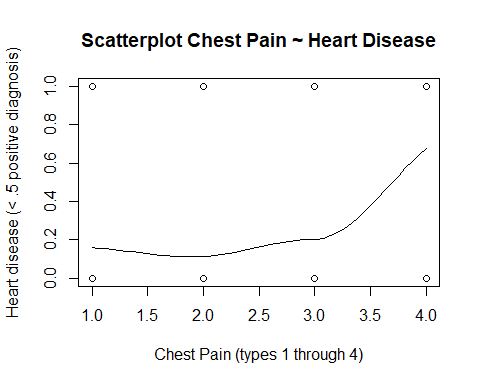
\includegraphics{project1_files/figure-latex/unnamed-chunk-4-1.pdf}

\begin{Shaded}
\begin{Highlighting}[]
\CommentTok{# # Density plot}
\KeywordTok{par}\NormalTok{(}\DataTypeTok{mfrow=}\KeywordTok{c}\NormalTok{(}\DecValTok{1}\NormalTok{, }\DecValTok{2}\NormalTok{))  }\CommentTok{# divide graph area in 2 columns}

\KeywordTok{plot}\NormalTok{(}\KeywordTok{density}\NormalTok{(df_hd}\OperatorTok{$}\NormalTok{cp), }\DataTypeTok{main=}\StringTok{"Density Plot: Chest Pain"}\NormalTok{, }\DataTypeTok{ylab=}\StringTok{"Frequency"}\NormalTok{, }\DataTypeTok{sub=}\KeywordTok{paste}\NormalTok{(}\StringTok{"Skewness:"}\NormalTok{, }\KeywordTok{round}\NormalTok{(e1071}\OperatorTok{::}\KeywordTok{skewness}\NormalTok{(df_hd}\OperatorTok{$}\NormalTok{cp), }\DecValTok{2}\NormalTok{)))}
\KeywordTok{polygon}\NormalTok{(}\KeywordTok{density}\NormalTok{(df_hd}\OperatorTok{$}\NormalTok{cp), }\DataTypeTok{col=}\StringTok{"red"}\NormalTok{)}

\KeywordTok{plot}\NormalTok{(}\KeywordTok{density}\NormalTok{(df_hd}\OperatorTok{$}\NormalTok{exang), }\DataTypeTok{main=}\StringTok{"Density Plot: Exercise induced CP"}\NormalTok{, }\DataTypeTok{ylab=}\StringTok{"Frequency"}\NormalTok{, }\DataTypeTok{sub=}\KeywordTok{paste}\NormalTok{(}\StringTok{"Skewness:"}\NormalTok{, }\KeywordTok{round}\NormalTok{(e1071}\OperatorTok{::}\KeywordTok{skewness}\NormalTok{(df_hd}\OperatorTok{$}\NormalTok{exang), }\DecValTok{2}\NormalTok{)))}
\KeywordTok{polygon}\NormalTok{(}\KeywordTok{density}\NormalTok{(df_hd}\OperatorTok{$}\NormalTok{exang), }\DataTypeTok{col=}\StringTok{"red"}\NormalTok{)}
\end{Highlighting}
\end{Shaded}

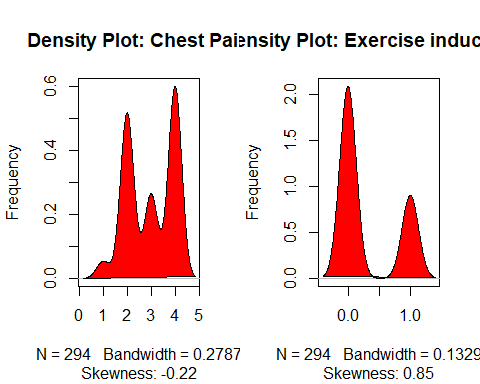
\includegraphics{project1_files/figure-latex/unnamed-chunk-4-2.pdf}

\section{first model for heart
disease}\label{first-model-for-heart-disease}

\section{This model uses exercise induced angina as the predictor for
the target of a heart disease
diagnosis}\label{this-model-uses-exercise-induced-angina-as-the-predictor-for-the-target-of-a-heart-disease-diagnosis}

The model has: Rsquared = .39 low pvalues for the predictor and target
low pvalue for the f-stastic

The rsquared value should be closer to 1, but this dataset is attempting
to predict something with alot of factors. So the nature of this data
explains why the rsquared value is low, it's complex.

When checking how the model does predicting on the test data. There is a
.69 correlation between the predicted value on the test data and the
training model. This model is a good represenation, not super duper, but
pretty good. I think this model performed well because the data set is
suited for linear regression.

\begin{Shaded}
\begin{Highlighting}[]
\CommentTok{# create linear model on train_data}
\NormalTok{train_lm1 <-}\StringTok{ }\KeywordTok{lm}\NormalTok{(}\KeywordTok{as.numeric}\NormalTok{(exang)}\OperatorTok{~}\KeywordTok{as.numeric}\NormalTok{(num), }\DataTypeTok{data=}\NormalTok{train_data)}
\KeywordTok{print}\NormalTok{(train_lm1 )}
\end{Highlighting}
\end{Shaded}

\begin{verbatim}
## 
## Call:
## lm(formula = as.numeric(exang) ~ as.numeric(num), data = train_data)
## 
## Coefficients:
##     (Intercept)  as.numeric(num)  
##          0.1212           0.5265
\end{verbatim}

\begin{Shaded}
\begin{Highlighting}[]
\KeywordTok{plot}\NormalTok{(train_lm1)}
\end{Highlighting}
\end{Shaded}

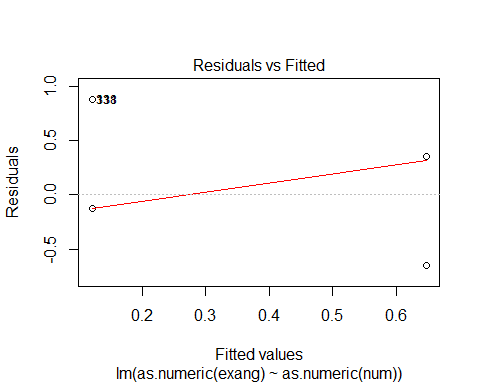
\includegraphics{project1_files/figure-latex/unnamed-chunk-5-1.pdf}
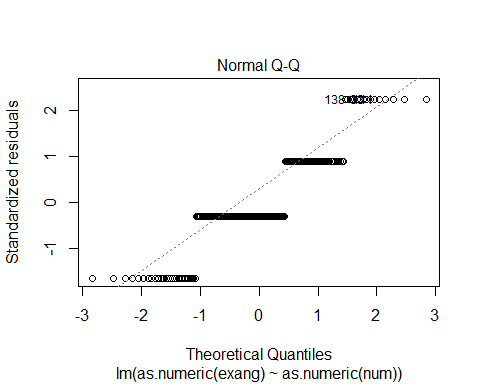
\includegraphics{project1_files/figure-latex/unnamed-chunk-5-2.pdf}
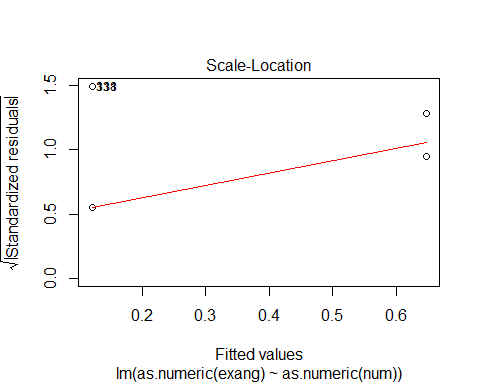
\includegraphics{project1_files/figure-latex/unnamed-chunk-5-3.pdf}
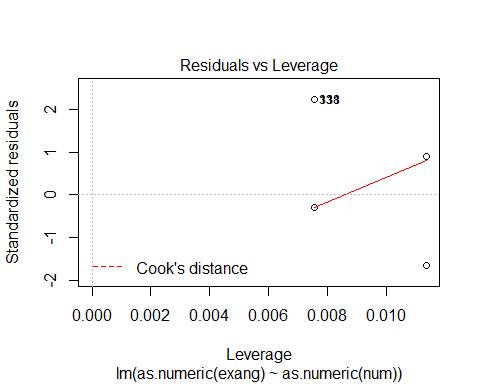
\includegraphics{project1_files/figure-latex/unnamed-chunk-5-4.pdf}

\begin{Shaded}
\begin{Highlighting}[]
\CommentTok{# store a summary of the model created from the train data and print it}
\NormalTok{lm1_sm <-}\StringTok{ }\KeywordTok{summary}\NormalTok{(train_lm1)}
\KeywordTok{print}\NormalTok{(lm1_sm)}
\end{Highlighting}
\end{Shaded}

\begin{verbatim}
## 
## Call:
## lm(formula = as.numeric(exang) ~ as.numeric(num), data = train_data)
## 
## Residuals:
##     Min      1Q  Median      3Q     Max 
## -0.6477 -0.1212 -0.1212  0.3523  0.8788 
## 
## Coefficients:
##                 Estimate Std. Error t value Pr(>|t|)    
## (Intercept)      0.12121    0.03444   3.519 0.000527 ***
## as.numeric(num)  0.52652    0.05446   9.668  < 2e-16 ***
## ---
## Signif. codes:  0 '***' 0.001 '**' 0.01 '*' 0.05 '.' 0.1 ' ' 1
## 
## Residual standard error: 0.3957 on 218 degrees of freedom
## Multiple R-squared:  0.3001, Adjusted R-squared:  0.2969 
## F-statistic: 93.46 on 1 and 218 DF,  p-value: < 2.2e-16
\end{verbatim}

\begin{Shaded}
\begin{Highlighting}[]
\CommentTok{# attempt to predict the target y value of the test data with the train linear model}
\NormalTok{pred <-}\StringTok{ }\KeywordTok{predict}\NormalTok{(train_lm1, }\DataTypeTok{newdata=}\NormalTok{test_data)}
\KeywordTok{print}\NormalTok{(}\StringTok{"Correlation of -- Prediction of heart disease using training model with test data:"}\NormalTok{)}
\end{Highlighting}
\end{Shaded}

\begin{verbatim}
## [1] "Correlation of -- Prediction of heart disease using training model with test data:"
\end{verbatim}

\begin{Shaded}
\begin{Highlighting}[]
\KeywordTok{cor}\NormalTok{(pred, }\KeywordTok{as.numeric}\NormalTok{(test_data}\OperatorTok{$}\NormalTok{exang))}
\end{Highlighting}
\end{Shaded}

\begin{verbatim}
## [1] 0.6968762
\end{verbatim}

\section{second model for heart
disease}\label{second-model-for-heart-disease}

\section{this model uses knn clustering with columns 9 and
10}\label{this-model-uses-knn-clustering-with-columns-9-and-10}

\section{exang and oldpeak to attempt to predict heart disease diagnosis
based on those two
predictors}\label{exang-and-oldpeak-to-attempt-to-predict-heart-disease-diagnosis-based-on-those-two-predictors}

correlation value of predictions vs actual: .66 this model was slightly
less accurate than the regression model. This data set is more suitable
towards linear regression models, so I think that's why this model is
less accurate since it uses classification when all of this data set is
numeric type.

\begin{Shaded}
\begin{Highlighting}[]
\CommentTok{# install and load packages}
\ControlFlowTok{if}\NormalTok{(}\OperatorTok{!}\KeywordTok{require}\NormalTok{(}\StringTok{'caret'}\NormalTok{))\{}
  \KeywordTok{install.packages}\NormalTok{(}\StringTok{'caret'}\NormalTok{)  }
  \KeywordTok{library}\NormalTok{(}\StringTok{'caret'}\NormalTok{)}
\NormalTok{\}}
\end{Highlighting}
\end{Shaded}

\begin{verbatim}
## Loading required package: caret
\end{verbatim}

\begin{verbatim}
## Loading required package: lattice
\end{verbatim}

\begin{verbatim}
## Loading required package: ggplot2
\end{verbatim}

\begin{Shaded}
\begin{Highlighting}[]
\ControlFlowTok{if}\NormalTok{(}\OperatorTok{!}\KeywordTok{require}\NormalTok{(}\StringTok{'DMwR'}\NormalTok{))\{}
  \KeywordTok{install.packages}\NormalTok{(}\StringTok{'DMwR'}\NormalTok{)  }
  \KeywordTok{library}\NormalTok{(}\StringTok{'DMwR'}\NormalTok{)}
\NormalTok{\}}
\end{Highlighting}
\end{Shaded}

\begin{verbatim}
## Loading required package: DMwR
\end{verbatim}

\begin{verbatim}
## Loading required package: grid
\end{verbatim}

\begin{Shaded}
\begin{Highlighting}[]
\CommentTok{# create the second linear model for heart disease data}
\NormalTok{train_lm2 <-}\StringTok{ }\KeywordTok{knnreg}\NormalTok{(train_data[,}\DecValTok{9}\OperatorTok{:}\DecValTok{10}\NormalTok{], train_data[,}\DecValTok{14}\NormalTok{], }\DataTypeTok{k=}\DecValTok{3}\NormalTok{)}

\CommentTok{# store a summary of the model created from the train data and print it}
\NormalTok{lm2_sm <-}\StringTok{ }\KeywordTok{summary}\NormalTok{(train_lm2)}
\KeywordTok{print}\NormalTok{(lm2_sm)}
\end{Highlighting}
\end{Shaded}

\begin{verbatim}
##         Length Class  Mode   
## learn   2      -none- list   
## k       1      -none- numeric
## theDots 0      -none- list
\end{verbatim}

\begin{Shaded}
\begin{Highlighting}[]
\CommentTok{# correlate how well the model did}
\CommentTok{# do this by comparing the performace of the model using test data for columns 9 and 10}
\CommentTok{# which are exang and oldpeak}
\CommentTok{# the model used those to predict heart disease based on those factors}
\NormalTok{predictions <-}\StringTok{ }\KeywordTok{predict}\NormalTok{(train_lm2, test_data[,}\DecValTok{9}\OperatorTok{:}\DecValTok{10}\NormalTok{])}
\CommentTok{# now correlate the predictions against the actual values in the test data}
\KeywordTok{print}\NormalTok{(}\StringTok{"Correlation of -- Prediction of heart disease using training model with test data:"}\NormalTok{)}
\end{Highlighting}
\end{Shaded}

\begin{verbatim}
## [1] "Correlation of -- Prediction of heart disease using training model with test data:"
\end{verbatim}

\begin{Shaded}
\begin{Highlighting}[]
\KeywordTok{cor}\NormalTok{(predictions, test_data}\OperatorTok{$}\NormalTok{num)}
\end{Highlighting}
\end{Shaded}

\begin{verbatim}
## [1] 0.6620159
\end{verbatim}

\section{Poker Hands}\label{poker-hands}

This data set is from the following URL:
\url{https://archive.ics.uci.edu/ml/datasets/Heart+Disease}

\begin{enumerate}
\def\labelenumi{\arabic{enumi})}
\item
  S1 ``Suit of card \#1'' Ordinal (1-4) representing \{Hearts, Spades,
  Diamonds, Clubs\}
\item
  C1 ``Rank of card \#1'' Numerical (1-13) representing (Ace, 2, 3,
  \ldots{} , Queen, King)
\item
  S2 ``Suit of card \#2'' Ordinal (1-4) representing \{Hearts, Spades,
  Diamonds, Clubs\}
\item
  C2 ``Rank of card \#2'' Numerical (1-13) representing (Ace, 2, 3,
  \ldots{} , Queen, King)
\item
  S3 ``Suit of card \#3'' Ordinal (1-4) representing \{Hearts, Spades,
  Diamonds, Clubs\}
\item
  C3 ``Rank of card \#3'' Numerical (1-13) representing (Ace, 2, 3,
  \ldots{} , Queen, King)
\item
  S4 ``Suit of card \#4'' Ordinal (1-4) representing \{Hearts, Spades,
  Diamonds, Clubs\}
\item
  C4 ``Rank of card \#4'' Numerical (1-13) representing (Ace, 2, 3,
  \ldots{} , Queen, King)
\item
  S5 ``Suit of card \#5'' Ordinal (1-4) representing \{Hearts, Spades,
  Diamonds, Clubs\}
\item
  C5 ``Rank of card 5'' Numerical (1-13) representing (Ace, 2, 3,
  \ldots{} , Queen, King)
\item
  CLASS ``Poker Hand'' Ordinal (0-9)
\end{enumerate}

0: Nothing in hand; not a recognized poker hand 1: One pair; one pair of
equal ranks within five cards 2: Two pairs; two pairs of equal ranks
within five cards 3: Three of a kind; three equal ranks within five
cards 4: Straight; five cards, sequentially ranked with no gaps 5:
Flush; five cards with the same suit 6: Full house; pair + different
rank three of a kind 7: Four of a kind; four equal ranks within five
cards 8: Straight flush; straight + flush 9: Royal flush; \{Ace, King,
Queen, Jack, Ten\} + flush

\section{load the project data for first set heart
disease}\label{load-the-project-data-for-first-set-heart-disease-1}

\begin{Shaded}
\begin{Highlighting}[]
\CommentTok{# different file locations for the project}
\NormalTok{dataPathHomeComputer <-}\StringTok{ "C:}\CharTok{\textbackslash{}\textbackslash{}}\StringTok{Users}\CharTok{\textbackslash{}\textbackslash{}}\StringTok{Alex}\CharTok{\textbackslash{}\textbackslash{}}\StringTok{Desktop}\CharTok{\textbackslash{}\textbackslash{}}\StringTok{Screen-Cleaner}\CharTok{\textbackslash{}\textbackslash{}}\StringTok{GitHub}\CharTok{\textbackslash{}\textbackslash{}}\StringTok{UTDSummer2018}\CharTok{\textbackslash{}\textbackslash{}}\StringTok{CS-4375.0U2-Machine-Learning}\CharTok{\textbackslash{}\textbackslash{}}\StringTok{Projects}\CharTok{\textbackslash{}\textbackslash{}}\StringTok{project1}\CharTok{\textbackslash{}\textbackslash{}}\StringTok{data}\CharTok{\textbackslash{}\textbackslash{}}\StringTok{processed.pokerhand.data"}

\NormalTok{dataPathSchoolComputer <-}\StringTok{ "H:}\CharTok{\textbackslash{}\textbackslash{}}\StringTok{GitHub}\CharTok{\textbackslash{}\textbackslash{}}\StringTok{UTDSummer2018}\CharTok{\textbackslash{}\textbackslash{}}\StringTok{CS-4375.0U2-Machine-Learning}\CharTok{\textbackslash{}\textbackslash{}}\StringTok{Projects}\CharTok{\textbackslash{}\textbackslash{}}\StringTok{project1}\CharTok{\textbackslash{}\textbackslash{}}\StringTok{data}\CharTok{\textbackslash{}\textbackslash{}}\StringTok{processed.pokerhand.data"}

\CommentTok{# create the dataframe for heart disease}
\NormalTok{df_ph <-}\StringTok{ }\KeywordTok{read.table}\NormalTok{(dataPathHomeComputer)}

\CommentTok{# sets the column names of the data frame with colnames function}
\KeywordTok{colnames}\NormalTok{(df_ph) <-}\StringTok{ }\KeywordTok{c}\NormalTok{(}\StringTok{"S1"}\NormalTok{,}\StringTok{"C1"}\NormalTok{,}\StringTok{"S2"}\NormalTok{,}\StringTok{"C2"}\NormalTok{,}\StringTok{"S3"}\NormalTok{,}\StringTok{"C3"}\NormalTok{,}\StringTok{"S4"}\NormalTok{,}\StringTok{"C4"}\NormalTok{,}\StringTok{"S5"}\NormalTok{,}\StringTok{"C5"}\NormalTok{,}\StringTok{"CLASS"}\NormalTok{)}



\CommentTok{# separate out the train and test dataframes following a similar naming convention of original frame}

\CommentTok{# Set random seed to ensure reproducibility of the shuffle.}
\KeywordTok{set.seed}\NormalTok{(}\DecValTok{1958}\NormalTok{)}


\CommentTok{# shuffle the df_ph and store into a new df_ph frame}
\NormalTok{df_ph_numberOfRows <-}\StringTok{ }\KeywordTok{nrow}\NormalTok{(df_ph)}
\NormalTok{shuf_df_ph <-}\StringTok{ }\NormalTok{df_ph[}\KeywordTok{sample}\NormalTok{(df_ph_numberOfRows), ]}

\CommentTok{# set train_ph_data df_ph with the train_ph_data indices}
\NormalTok{train_ph_data_indices <-}\StringTok{ }\DecValTok{1}\OperatorTok{:}\KeywordTok{round}\NormalTok{(}\FloatTok{0.75} \OperatorTok{*}\StringTok{ }\NormalTok{df_ph_numberOfRows)}
\NormalTok{train_ph_data <-}\StringTok{ }\NormalTok{shuf_df_ph[train_ph_data_indices, ]}
\CommentTok{# set test_ph_data df_ph with the test_ph_data indices}
\NormalTok{test_ph_data_indices <-}\StringTok{ }\NormalTok{(}\KeywordTok{round}\NormalTok{(}\FloatTok{0.75} \OperatorTok{*}\StringTok{ }\NormalTok{df_ph_numberOfRows) }\OperatorTok{+}\StringTok{ }\DecValTok{1}\NormalTok{)}\OperatorTok{:}\NormalTok{df_ph_numberOfRows}
\NormalTok{test_ph_data <-}\StringTok{ }\NormalTok{shuf_df_ph[test_ph_data_indices, ]}
\end{Highlighting}
\end{Shaded}

\section{investigate the data with names, str, head, summary and
cor}\label{investigate-the-data-with-names-str-head-summary-and-cor-1}

\begin{Shaded}
\begin{Highlighting}[]
\CommentTok{# look at the names of the data frame}
\NormalTok{nameArray <-}\StringTok{ }\KeywordTok{names}\NormalTok{(df_ph)}
\NormalTok{printString <-}\StringTok{ "The names of the columns are:"}

\CommentTok{# print a useful message with a compact version of the columns using str}
\KeywordTok{print}\NormalTok{(printString)}
\end{Highlighting}
\end{Shaded}

\begin{verbatim}
## [1] "The names of the columns are:"
\end{verbatim}

\begin{Shaded}
\begin{Highlighting}[]
\KeywordTok{str}\NormalTok{(nameArray)}
\end{Highlighting}
\end{Shaded}

\begin{verbatim}
##  chr [1:11] "S1" "C1" "S2" "C2" "S3" "C3" "S4" "C4" "S5" "C5" "CLASS"
\end{verbatim}

\begin{Shaded}
\begin{Highlighting}[]
\CommentTok{# show first 6 instances of the frame}
\KeywordTok{head}\NormalTok{(df_ph)}
\end{Highlighting}
\end{Shaded}

\begin{verbatim}
##   S1 C1 S2 C2 S3 C3 S4 C4 S5 C5 CLASS
## 1  1  1  1 13  2  4  2  3  1 12     0
## 2  3 12  3  2  3 11  4  5  2  5     1
## 3  1  9  4  6  1  4  3  2  3  9     1
## 4  1  4  3 13  2 13  2  1  3  6     1
## 5  3 10  2  7  1  2  2 11  4  9     0
## 6  1  3  4  5  3  4  1 12  4  6     0
\end{verbatim}

None of the indivudal columns correlated well with the Royal Flush hand
classification: all were under .015

\begin{Shaded}
\begin{Highlighting}[]
\CommentTok{# store a summary of the data frame}
\NormalTok{sm <-}\StringTok{ }\KeywordTok{summary}\NormalTok{(df_ph)}

\CommentTok{# print the summary}
\KeywordTok{print}\NormalTok{(sm)}
\end{Highlighting}
\end{Shaded}

\begin{verbatim}
##        S1            C1               S2              C2        
##  Min.   :1.0   Min.   : 1.000   Min.   :1.000   Min.   : 1.000  
##  1st Qu.:2.0   1st Qu.: 4.000   1st Qu.:1.000   1st Qu.: 4.000  
##  Median :2.0   Median : 7.000   Median :2.000   Median : 7.000  
##  Mean   :2.5   Mean   : 6.935   Mean   :2.471   Mean   : 7.024  
##  3rd Qu.:3.0   3rd Qu.:10.000   3rd Qu.:3.000   3rd Qu.:10.000  
##  Max.   :4.0   Max.   :13.000   Max.   :4.000   Max.   :13.000  
##        S3              C3               S4              C4        
##  Min.   :1.000   Min.   : 1.000   Min.   :1.000   Min.   : 1.000  
##  1st Qu.:2.000   1st Qu.: 4.000   1st Qu.:2.000   1st Qu.: 4.000  
##  Median :3.000   Median : 7.000   Median :3.000   Median : 7.000  
##  Mean   :2.512   Mean   : 6.945   Mean   :2.506   Mean   : 6.933  
##  3rd Qu.:4.000   3rd Qu.:10.000   3rd Qu.:4.000   3rd Qu.:10.000  
##  Max.   :4.000   Max.   :13.000   Max.   :4.000   Max.   :13.000  
##        S5              C5             CLASS       
##  Min.   :1.000   Min.   : 1.000   Min.   :0.0000  
##  1st Qu.:2.000   1st Qu.: 4.000   1st Qu.:0.0000  
##  Median :3.000   Median : 7.000   Median :0.0000  
##  Mean   :2.522   Mean   : 6.994   Mean   :0.6244  
##  3rd Qu.:4.000   3rd Qu.:10.000   3rd Qu.:1.0000  
##  Max.   :4.000   Max.   :13.000   Max.   :7.0000
\end{verbatim}

\begin{Shaded}
\begin{Highlighting}[]
\CommentTok{# coerce all predictors and targets as numeric for correlation function}

\NormalTok{xPredictor <-}\StringTok{ }\KeywordTok{as.numeric}\NormalTok{(df_ph}\OperatorTok{$}\NormalTok{C1)}
\NormalTok{yTarget <-}\StringTok{ }\KeywordTok{as.numeric}\NormalTok{(df_ph}\OperatorTok{$}\NormalTok{CLASS)}

\KeywordTok{print}\NormalTok{(}\StringTok{"Correlation of -- Card 1 value and Hand Classfication:"}\NormalTok{)}
\end{Highlighting}
\end{Shaded}

\begin{verbatim}
## [1] "Correlation of -- Card 1 value and Hand Classfication:"
\end{verbatim}

\begin{Shaded}
\begin{Highlighting}[]
\KeywordTok{cor}\NormalTok{(xPredictor, yTarget)}
\end{Highlighting}
\end{Shaded}

\begin{verbatim}
## [1] -0.01236034
\end{verbatim}

\begin{Shaded}
\begin{Highlighting}[]
\NormalTok{xPredictor <-}\StringTok{ }\KeywordTok{as.numeric}\NormalTok{(df_ph}\OperatorTok{$}\NormalTok{S1)}
\KeywordTok{print}\NormalTok{(}\StringTok{"Correlation of -- Card 1 suit and Hand Classfication:"}\NormalTok{)}
\end{Highlighting}
\end{Shaded}

\begin{verbatim}
## [1] "Correlation of -- Card 1 suit and Hand Classfication:"
\end{verbatim}

\begin{Shaded}
\begin{Highlighting}[]
\KeywordTok{cor}\NormalTok{(xPredictor, yTarget)}
\end{Highlighting}
\end{Shaded}

\begin{verbatim}
## [1] -0.01133808
\end{verbatim}

\begin{Shaded}
\begin{Highlighting}[]
\NormalTok{xPredictor <-}\StringTok{ }\KeywordTok{as.numeric}\NormalTok{(df_ph}\OperatorTok{$}\NormalTok{C3)}
\KeywordTok{print}\NormalTok{(}\StringTok{"Correlation of -- Card 3 and Hand Classfication:"}\NormalTok{)}
\end{Highlighting}
\end{Shaded}

\begin{verbatim}
## [1] "Correlation of -- Card 3 and Hand Classfication:"
\end{verbatim}

\begin{Shaded}
\begin{Highlighting}[]
\KeywordTok{cor}\NormalTok{(xPredictor, yTarget)}
\end{Highlighting}
\end{Shaded}

\begin{verbatim}
## [1] 0.01405256
\end{verbatim}

\begin{Shaded}
\begin{Highlighting}[]
\NormalTok{xPredictor <-}\StringTok{ }\KeywordTok{as.numeric}\NormalTok{(df_ph}\OperatorTok{$}\NormalTok{S3)}
\KeywordTok{print}\NormalTok{(}\StringTok{"Correlation of --  Card 3 suit and Hand Classfication:"}\NormalTok{)}
\end{Highlighting}
\end{Shaded}

\begin{verbatim}
## [1] "Correlation of --  Card 3 suit and Hand Classfication:"
\end{verbatim}

\begin{Shaded}
\begin{Highlighting}[]
\KeywordTok{cor}\NormalTok{(xPredictor, yTarget)}
\end{Highlighting}
\end{Shaded}

\begin{verbatim}
## [1] 0.004862796
\end{verbatim}

\section{two informative graphs}\label{two-informative-graphs-1}

The scatter plot shows the likelyhood of hand classfication based on
card 1 value The scatter plot shows that there is no correlation between
the two

The density plots show the distribution of certain predictors in the
data set. In this case I chose card 1 value and card 1 suit. The
predictors are very normally distributed.

\begin{Shaded}
\begin{Highlighting}[]
\CommentTok{# scatterplot for data view}
\KeywordTok{scatter.smooth}\NormalTok{(}\DataTypeTok{x=}\NormalTok{df_ph}\OperatorTok{$}\NormalTok{C1, }\DataTypeTok{y=}\NormalTok{df_ph}\OperatorTok{$}\NormalTok{CLASS, }\DataTypeTok{main=}\StringTok{"Card 1 value ~ Hand Classfication"}\NormalTok{, }\DataTypeTok{xlab=}\StringTok{"Card 1 value"}\NormalTok{, }\DataTypeTok{ylab=}\StringTok{"Hand classification (0 nothing - 9 Royal Flush"}\NormalTok{)}
\end{Highlighting}
\end{Shaded}

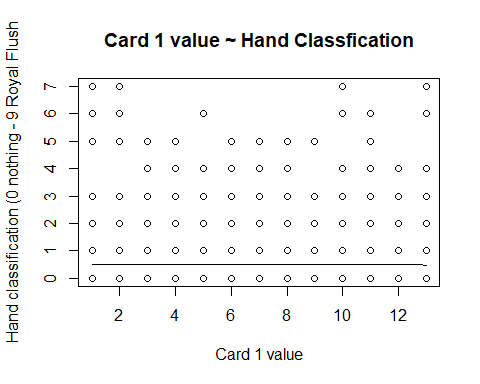
\includegraphics{project1_files/figure-latex/unnamed-chunk-10-1.pdf}

\begin{Shaded}
\begin{Highlighting}[]
\CommentTok{#pairs plot}
\KeywordTok{pairs}\NormalTok{(df_ph)}
\end{Highlighting}
\end{Shaded}

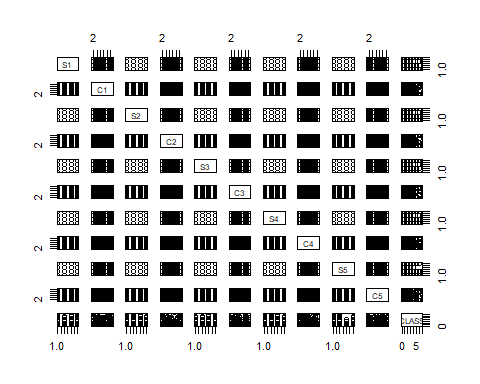
\includegraphics{project1_files/figure-latex/unnamed-chunk-10-2.pdf}

\begin{Shaded}
\begin{Highlighting}[]
\CommentTok{# # Density plot}
\KeywordTok{par}\NormalTok{(}\DataTypeTok{mfrow=}\KeywordTok{c}\NormalTok{(}\DecValTok{1}\NormalTok{, }\DecValTok{2}\NormalTok{))  }\CommentTok{# divide graph area in 2 columns}

\KeywordTok{plot}\NormalTok{(}\KeywordTok{density}\NormalTok{(df_ph}\OperatorTok{$}\NormalTok{C1), }\DataTypeTok{main=}\StringTok{"Density Plot: Card 1 value"}\NormalTok{, }\DataTypeTok{ylab=}\StringTok{"Frequency"}\NormalTok{, }\DataTypeTok{sub=}\KeywordTok{paste}\NormalTok{(}\StringTok{"Skewness:"}\NormalTok{, }\KeywordTok{round}\NormalTok{(e1071}\OperatorTok{::}\KeywordTok{skewness}\NormalTok{(df_ph}\OperatorTok{$}\NormalTok{C1), }\DecValTok{2}\NormalTok{)))}
\KeywordTok{polygon}\NormalTok{(}\KeywordTok{density}\NormalTok{(df_ph}\OperatorTok{$}\NormalTok{C1), }\DataTypeTok{col=}\StringTok{"red"}\NormalTok{)}

\KeywordTok{plot}\NormalTok{(}\KeywordTok{density}\NormalTok{(df_ph}\OperatorTok{$}\NormalTok{S1), }\DataTypeTok{main=}\StringTok{"Density Plot: Card 1 suit"}\NormalTok{, }\DataTypeTok{ylab=}\StringTok{"Frequency"}\NormalTok{, }\DataTypeTok{sub=}\KeywordTok{paste}\NormalTok{(}\StringTok{"Skewness:"}\NormalTok{, }\KeywordTok{round}\NormalTok{(e1071}\OperatorTok{::}\KeywordTok{skewness}\NormalTok{(df_ph}\OperatorTok{$}\NormalTok{S1), }\DecValTok{2}\NormalTok{)))}
\KeywordTok{polygon}\NormalTok{(}\KeywordTok{density}\NormalTok{(df_ph}\OperatorTok{$}\NormalTok{S1), }\DataTypeTok{col=}\StringTok{"red"}\NormalTok{)}
\end{Highlighting}
\end{Shaded}

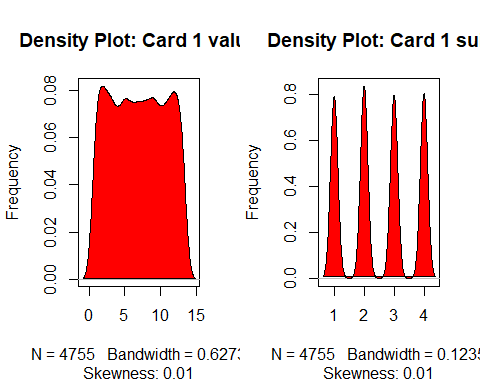
\includegraphics{project1_files/figure-latex/unnamed-chunk-10-3.pdf}

\section{first model for heart
disease}\label{first-model-for-heart-disease-1}

\section{This model uses exercise induced angina as the predictor for
the target of a heart disease
diagnosis}\label{this-model-uses-exercise-induced-angina-as-the-predictor-for-the-target-of-a-heart-disease-diagnosis-1}

The model has: Rsquared = .000 low pvalues for the predictor high pvalue
for the target low pvalue for the f-stastic

The rsquared value shows this regression technique explains none of the
variance in the predictors. So the nature of this data explains why the
rsquared value is low. This data set is not intended for regression

\begin{Shaded}
\begin{Highlighting}[]
\CommentTok{# create linear model on train_ph_data}
\NormalTok{train_lm1_ph <-}\StringTok{ }\KeywordTok{lm}\NormalTok{(df_ph}\OperatorTok{$}\NormalTok{C1}\OperatorTok{~}\NormalTok{df_ph}\OperatorTok{$}\NormalTok{CLASS, }\DataTypeTok{data=}\NormalTok{train_ph_data)}
\KeywordTok{print}\NormalTok{(train_lm1_ph)}
\end{Highlighting}
\end{Shaded}

\begin{verbatim}
## 
## Call:
## lm(formula = df_ph$C1 ~ df_ph$CLASS, data = train_ph_data)
## 
## Coefficients:
## (Intercept)  df_ph$CLASS  
##     6.97082     -0.05802
\end{verbatim}

\begin{Shaded}
\begin{Highlighting}[]
\KeywordTok{plot}\NormalTok{(train_lm1_ph)}
\end{Highlighting}
\end{Shaded}

\includegraphics{project1_files/figure-latex/unnamed-chunk-11-1.pdf}
\includegraphics{project1_files/figure-latex/unnamed-chunk-11-2.pdf}
\includegraphics{project1_files/figure-latex/unnamed-chunk-11-3.pdf}
\includegraphics{project1_files/figure-latex/unnamed-chunk-11-4.pdf}

\begin{Shaded}
\begin{Highlighting}[]
\CommentTok{# store a summary of the model created from the train data and print it}
\NormalTok{lm1_ph_sm <-}\StringTok{ }\KeywordTok{summary}\NormalTok{(train_lm1_ph)}
\KeywordTok{print}\NormalTok{(lm1_ph_sm)}
\end{Highlighting}
\end{Shaded}

\begin{verbatim}
## 
## Call:
## lm(formula = df_ph$C1 ~ df_ph$CLASS, data = train_ph_data)
## 
## Residuals:
##     Min      1Q  Median      3Q     Max 
## -5.9708 -2.9708  0.0292  3.0872  6.4353 
## 
## Coefficients:
##             Estimate Std. Error t value Pr(>|t|)    
## (Intercept)  6.97082    0.06948 100.322   <2e-16 ***
## df_ph$CLASS -0.05802    0.06808  -0.852    0.394    
## ---
## Signif. codes:  0 '***' 0.001 '**' 0.01 '*' 0.05 '.' 0.1 ' ' 1
## 
## Residual standard error: 3.79 on 4753 degrees of freedom
## Multiple R-squared:  0.0001528,  Adjusted R-squared:  -5.758e-05 
## F-statistic: 0.7263 on 1 and 4753 DF,  p-value: 0.3941
\end{verbatim}

\section{second model for poker card
hand}\label{second-model-for-poker-card-hand}

\section{this model uses logistic regression to attempt to predict hand
classification from card values and
suits}\label{this-model-uses-logistic-regression-to-attempt-to-predict-hand-classification-from-card-values-and-suits}

the accuracy is .5 which is alot higher than the regression used in the
previous model

this data set is more geared towards classification, so that explains
why logistic regression did better.

\begin{Shaded}
\begin{Highlighting}[]
\CommentTok{# scale the value which determines the hand classification so it ranges between .1 and .9}
\CommentTok{# this allows glm to work on the y value}
\NormalTok{train_ph_data[,}\DecValTok{11}\NormalTok{]<-train_ph_data[,}\DecValTok{11}\NormalTok{]}\OperatorTok{*}\NormalTok{.}\DecValTok{1}
\NormalTok{test_ph_data[,}\DecValTok{11}\NormalTok{]<-test_ph_data[,}\DecValTok{11}\NormalTok{]}\OperatorTok{*}\NormalTok{.}\DecValTok{1}

\NormalTok{train_lm2_ph <-}\StringTok{ }\KeywordTok{glm}\NormalTok{(CLASS}\OperatorTok{~}\NormalTok{., }\DataTypeTok{data=}\NormalTok{train_ph_data, }\DataTypeTok{family=}\StringTok{"binomial"}\NormalTok{)}
\end{Highlighting}
\end{Shaded}

\begin{verbatim}
## Warning in eval(family$initialize): non-integer #successes in a binomial
## glm!
\end{verbatim}

\begin{Shaded}
\begin{Highlighting}[]
\CommentTok{# store a summary of the model created from the train data and print it}
\NormalTok{lm2_ph_sm <-}\StringTok{ }\KeywordTok{summary}\NormalTok{(train_lm2_ph)}
\KeywordTok{print}\NormalTok{(lm2_ph_sm)}
\end{Highlighting}
\end{Shaded}

\begin{verbatim}
## 
## Call:
## glm(formula = CLASS ~ ., family = "binomial", data = train_ph_data)
## 
## Deviance Residuals: 
##     Min       1Q   Median       3Q      Max  
## -0.4002  -0.3585  -0.3297   0.1483   1.6094  
## 
## Coefficients:
##               Estimate Std. Error z value Pr(>|z|)    
## (Intercept) -2.3799397  0.4655810  -5.112 3.19e-07 ***
## S1          -0.0219364  0.0624395  -0.351    0.725    
## C1          -0.0036185  0.0182600  -0.198    0.843    
## S2          -0.0307575  0.0620979  -0.495    0.620    
## C2          -0.0122942  0.0185530  -0.663    0.508    
## S3           0.0022338  0.0616806   0.036    0.971    
## C3           0.0030229  0.0184489   0.164    0.870    
## S4          -0.0014471  0.0619946  -0.023    0.981    
## C4          -0.0044036  0.0184200  -0.239    0.811    
## S5          -0.0296658  0.0621843  -0.477    0.633    
## C5          -0.0008516  0.0188071  -0.045    0.964    
## ---
## Signif. codes:  0 '***' 0.001 '**' 0.01 '*' 0.05 '.' 0.1 ' ' 1
## 
## (Dispersion parameter for binomial family taken to be 1)
## 
##     Null deviance: 389.06  on 3565  degrees of freedom
## Residual deviance: 387.93  on 3555  degrees of freedom
## AIC: 546.36
## 
## Number of Fisher Scoring iterations: 5
\end{verbatim}

\begin{Shaded}
\begin{Highlighting}[]
\NormalTok{probs <-}\StringTok{ }\KeywordTok{predict}\NormalTok{(train_lm2_ph, }\DataTypeTok{newdata=}\NormalTok{test_ph_data)}
\NormalTok{pred <-}\StringTok{ }\KeywordTok{ifelse}\NormalTok{(probs}\OperatorTok{>}\FloatTok{0.0}\NormalTok{, }\FloatTok{0.9}\NormalTok{, }\DecValTok{0}\NormalTok{)}
\NormalTok{acc <-}\StringTok{ }\KeywordTok{mean}\NormalTok{(pred}\OperatorTok{==}\NormalTok{test_ph_data}\OperatorTok{$}\NormalTok{CLASS)}
\KeywordTok{print}\NormalTok{(}\KeywordTok{paste}\NormalTok{(}\StringTok{"accuracy = "}\NormalTok{, acc))}
\end{Highlighting}
\end{Shaded}

\begin{verbatim}
## [1] "accuracy =  0.507148864592094"
\end{verbatim}

\begin{Shaded}
\begin{Highlighting}[]
\KeywordTok{table}\NormalTok{(pred, test_ph_data}\OperatorTok{$}\NormalTok{CLASS) }
\end{Highlighting}
\end{Shaded}

\begin{verbatim}
##     
## pred   0 0.1 0.2 0.3 0.4 0.5 0.7
##    0 603 488  58  27  11   1   1
\end{verbatim}


\end{document}
